% !TeX root = ../main.tex

\chapter{相关工作}\label{cha:related_work}
\section{视觉推理}\label{sec:visural_reasoning}
到目前为止,学者们已经提出了许多种视觉推理任务,视觉问答(Visual Question Answering, VQA)\cite{antol2015vqa}是其中比较早的一类任务。在VQA任务中,模型的输入是一张图片和一个与图片相关的问题,模型需要根据图片中的内容来回答问题。图~\ref{fig:vqa}~是VQA数据集\cite{antol2015vqa}中的一些例子。
\begin{figure}[!b]
    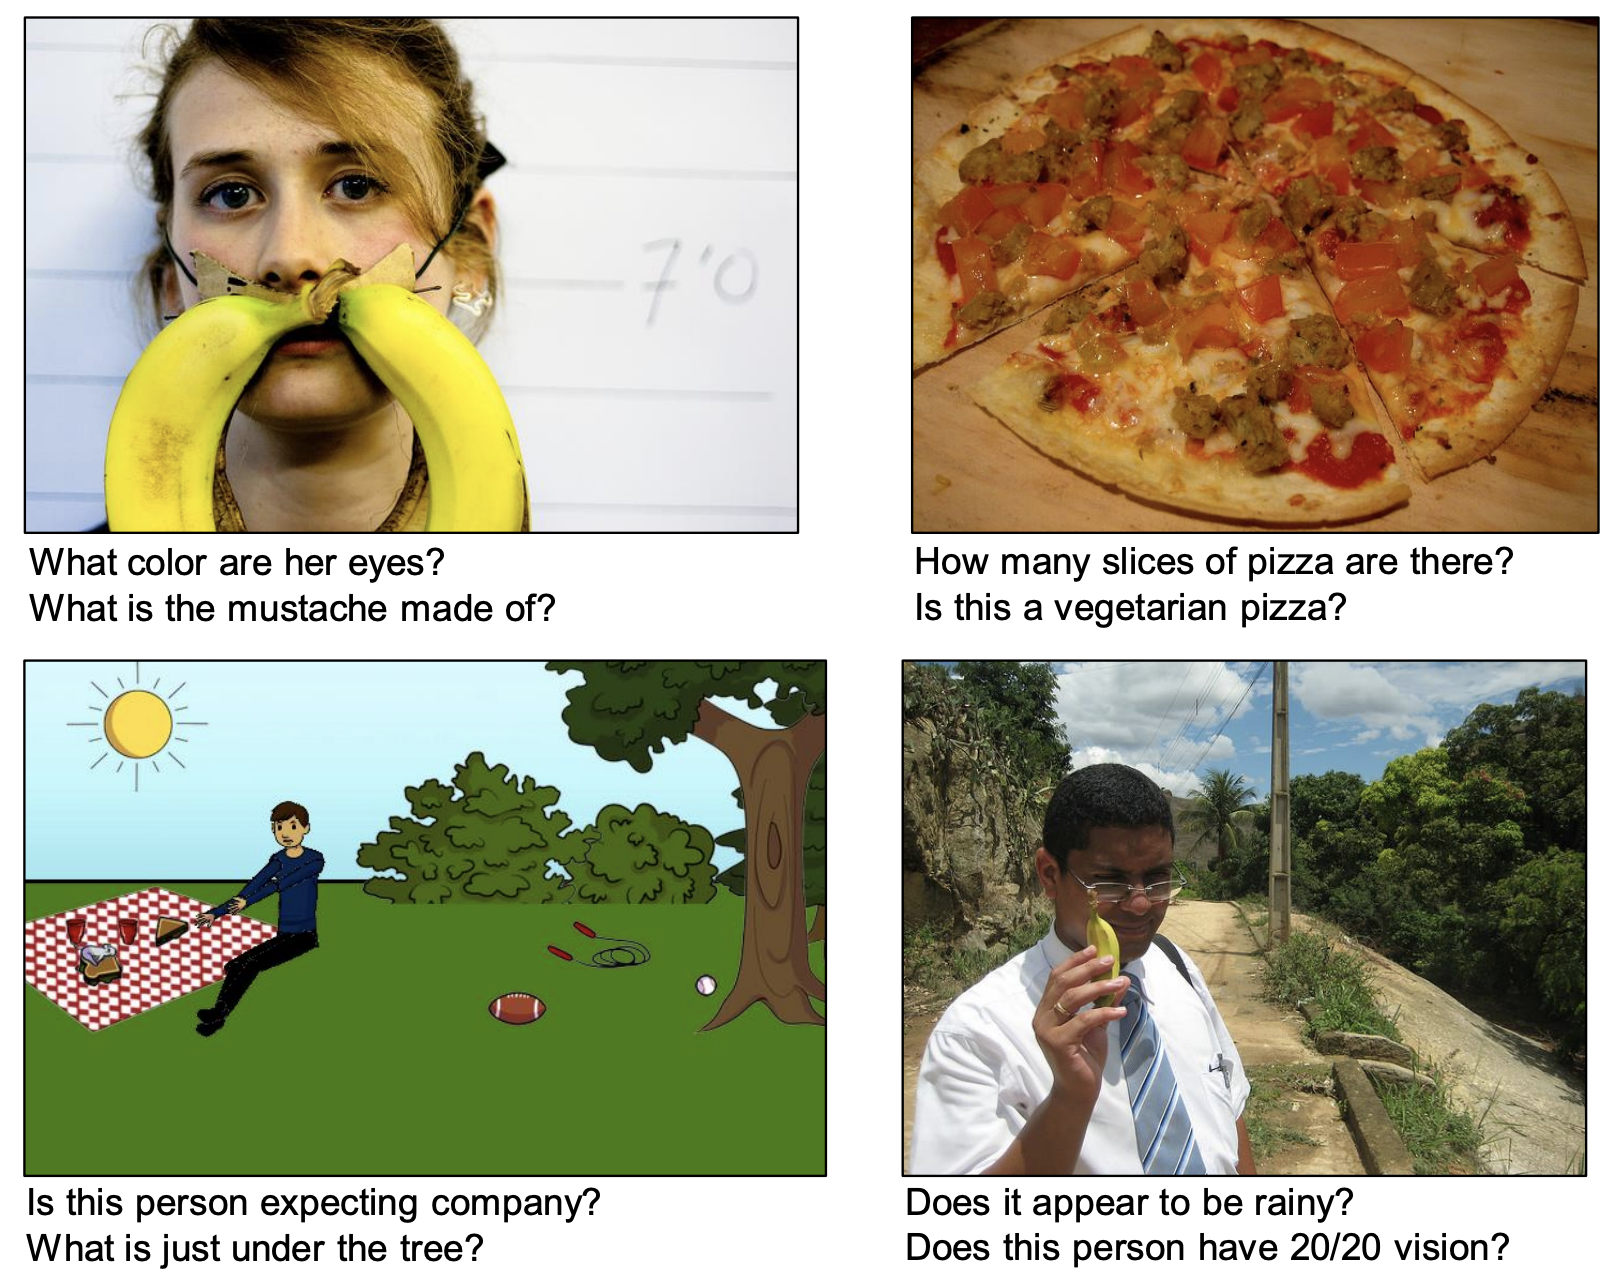
\includegraphics[width = \textwidth]{vqa.png}
    \caption{VQA数据集}
    \label{fig:vqa}
\end{figure}
可以看到,VQA数据集中的图片来自于真实世界中的场景,其对应的问题也具有多样性。

然而,VQA\cite{antol2015vqa}数据集是严重有偏的。例如,对于以``Do you see
a...''开头的问题,模型不看图片直接回答``yes''就可以获得87\%的准确率\cite{goyal2017making}。也就是说,在有些情况下,模型掌握了一些捷径,从而可以无需关注图片的内容,甚至不用读完问题,就可以取得正确的答案。为了解决这个问题,Goyal~\etal\cite{goyal2017making}提出了在 VQA 数据集的基础上构建平衡的数据集,得到了改进版本:VQAv2.0。VQAv2.0 中的每个问题都对应着两张图片,并确保在这两张图片上该问题的答案不同,如图~\ref{fig:vqav2}~所示。这样的设计保证了模型不可能仅仅根据问题就得出答案,从而必须对视觉信息进行推理。在VQAv2.0上表现较好的模型总体上的架构类似\cite{kim2018bilinear,anderson2018bottom,gao2019dynamic},其关键在于视觉特征和文本特征的提取和融合。在特征提取方面,这些模型通常使用目标检测中的R-CNN\cite{ren2015faster}模型来提取视觉特征,利用循环神经网络(LSTM\cite{hochreiter1997long}、GRU\cite{cho2014learning})来提取文本特征。得到了视觉和文本特征后,可以采用多种方法完成特征的融合。例如,Kim~\etal\cite{kim2018bilinear}使用双线性注意力网络来融合特征;Anderson~\etal\cite{anderson2018bottom}首先用文本特征计算注意力系数来对图像特征加权,再将两种特征融合;Gao~\etal\cite{gao2019dynamic}则综合使用模态内和模态间的动态注意力机制将视觉特征和文本特征逐步融合。然而,这些基于视觉特征和文本特征的提取和融合的方法都缺乏对推理过程的建模。

\begin{figure}
    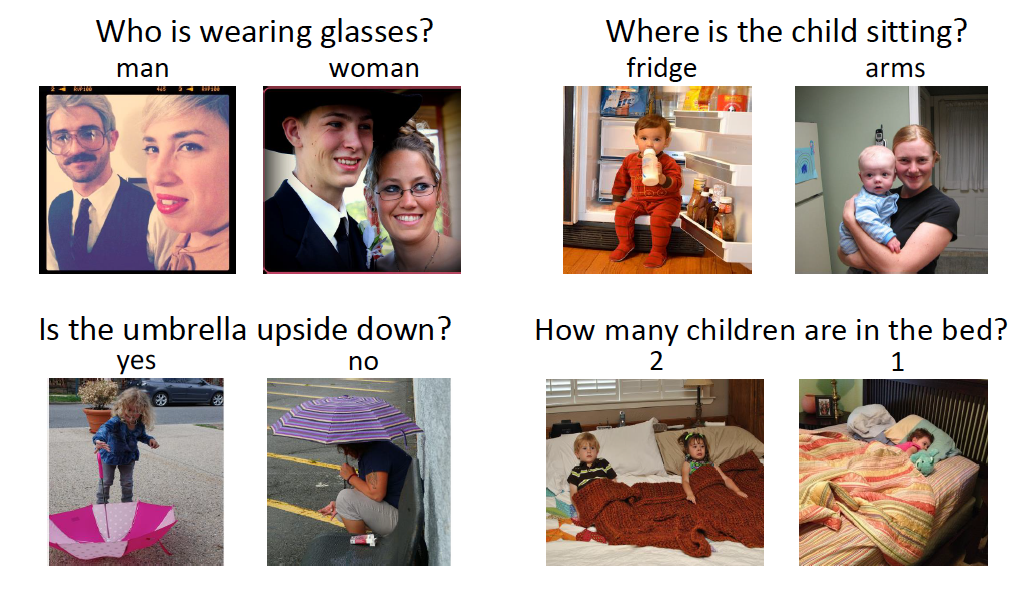
\includegraphics[width = \textwidth]{vqav2.png}
    \caption{VQAv2.0数据集\cite{goyal2017making}}
    \label{fig:vqav2}
\end{figure}

为了对深度模型执行推理的能力进行诊断,Johnson~\etal 提出了CLEVR数据集\cite{johnson2017clevr},如图~\ref{fig:clevr}~所示。CLEVR数据集中的图片由许多简单的、具有不同属性的三维图形构成,每个图片都通过一个场景图渲染而来;通过深度优先搜索,并利用场景图剪枝,可以构建出一系列满足要求的问题以及与之对应的答案。同时,每一个问题都可以表示称一个程序。在已知场景图和程序的情况下,逐步执行程序即可得到正确的答案。这就带来了另外一个问题:推理的过程已经蕴含在问题的自然语言中,从而降低了对模型的推理能力的要求。事实上,许多工作的重点都放在了如何从自然语言生成其对应的程序。例如,Johnson~\etal\cite{Johnson_2017_ICCV} 使用程序生成网络从问题生成程序,再使用神经模块网络\cite{andreas2016neural}搭建执行引擎来执行这个程序。Yi~\etal\cite{yi2018neural} 则将神经网络和符号计算相结合,首先用Mask R-CNN\cite{he2017mask}解析出图片场景中的各种元素的属性,再用LSTM\cite{hochreiter1997long}从问题生成程序,最后直接使用符号计算的方法执行该程序得到答案。Shi~\etal\cite{shi2019explainable} 提出了用神经网络在图片上反推出场景图,再在场景图上执行程序。在这些方法中,自然语言都起到了主导的作用,也就是说模型通过自然语言就可以显示或隐式地得到了推理的过程。相比于这一类问题,我们更希望有一种纯视觉推理任务。

\begin{figure}
    \centering
    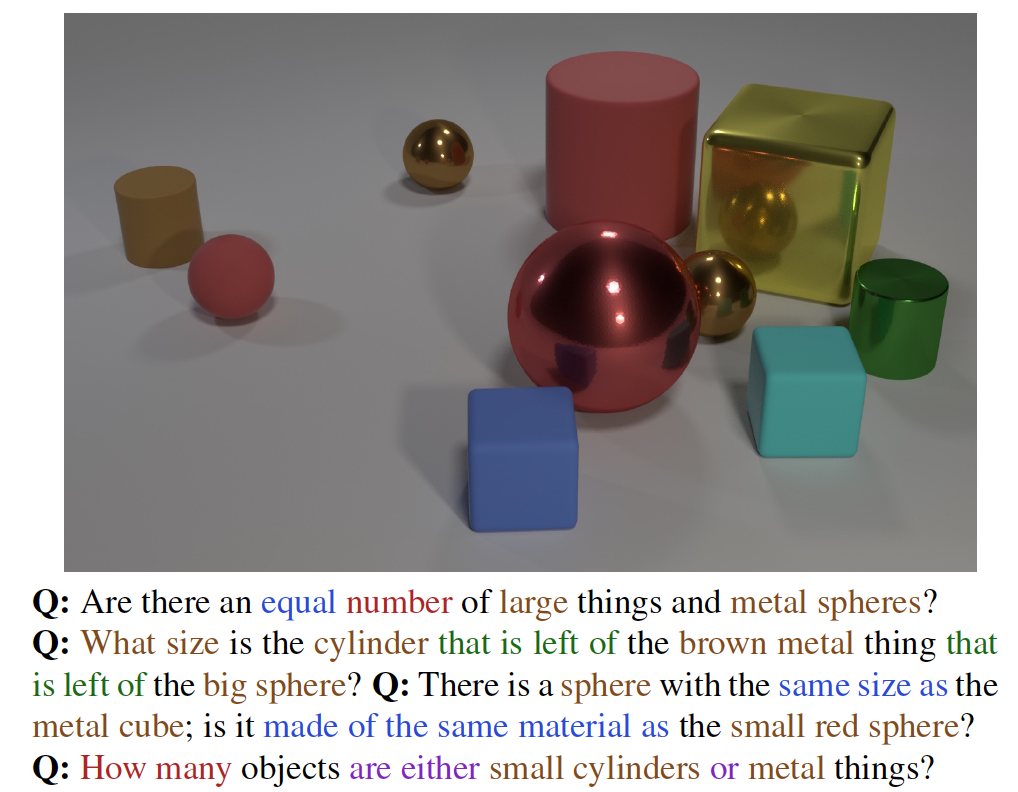
\includegraphics[width=0.8\textwidth]{clevr.png}
    \caption{CLEVR 数据集\cite{johnson2017clevr}}
    \label{fig:clevr}
\end{figure}

另一类视觉推理任务称为抽象推理(Abstract Reasoning)\cite{barrett2018measuring,zhang2019raven}。这类任务建立在瑞文推理测验(Raven Progressive Matrices, RPM)上。RAVEN数据集\cite{zhang2019raven}就是其中一个例子,如图~\ref{fig:raven}~所示。RPM中的问题是一个$3\times 3$的矩阵,其中8张图片已知,一张图片未知。已知的图片在行列上存在一定的规律,例如图片中图形颜色、形状、个数、排列方式的变化等等。模型需要找到这些规律,并从候选的答案集合里选出最合适的选项。虽然这个任务中没有自然语言的干扰,但由于这里的问题和选项都是人工合成的简单图片,该任务更像是一些智力测试题,而难以有实际的应用。另一方面,一些简单的模型反而能够在这个任务上取得很好的效果。例如,仅仅将所有图片拼接在一起作为输入,经过一个ResNet18\cite{he2016deep}分类就可以达到比原论文\cite{zhang2019raven}中更好的结果。

\begin{figure}
    \centering
    \begin{subfigure}{.35\textwidth}
        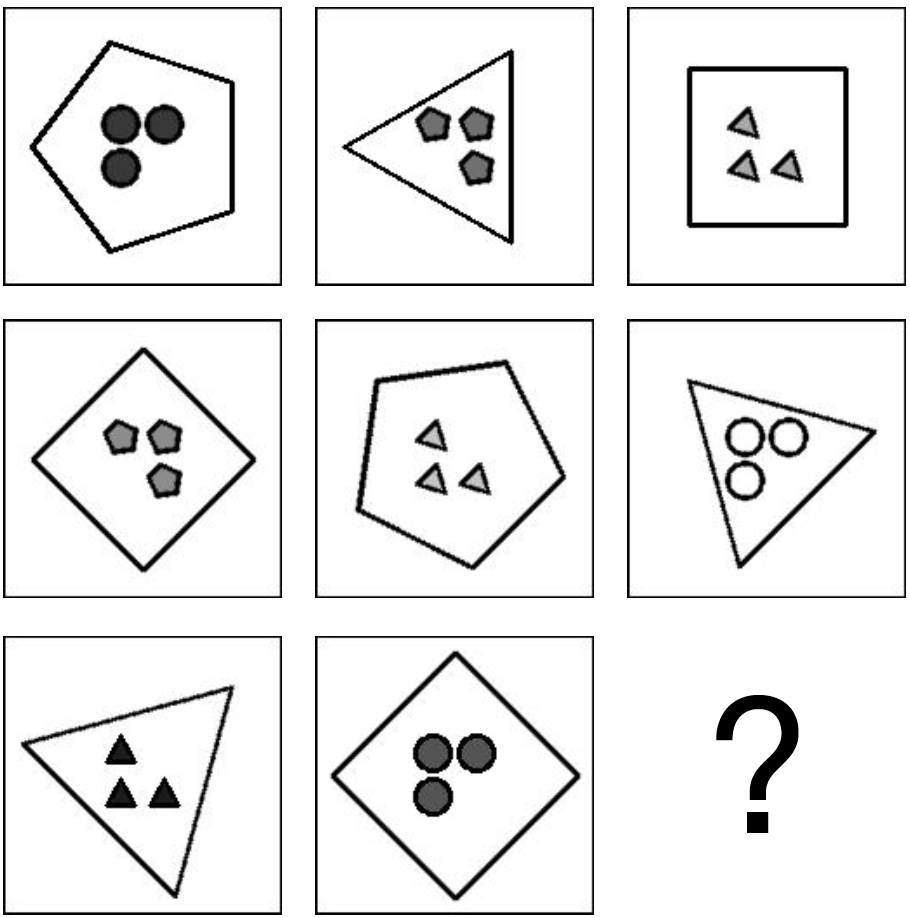
\includegraphics[width=\textwidth]{raven1.png}
        \caption{问题}
    \end{subfigure}\hfill
    \begin{subfigure}{.55\textwidth}
        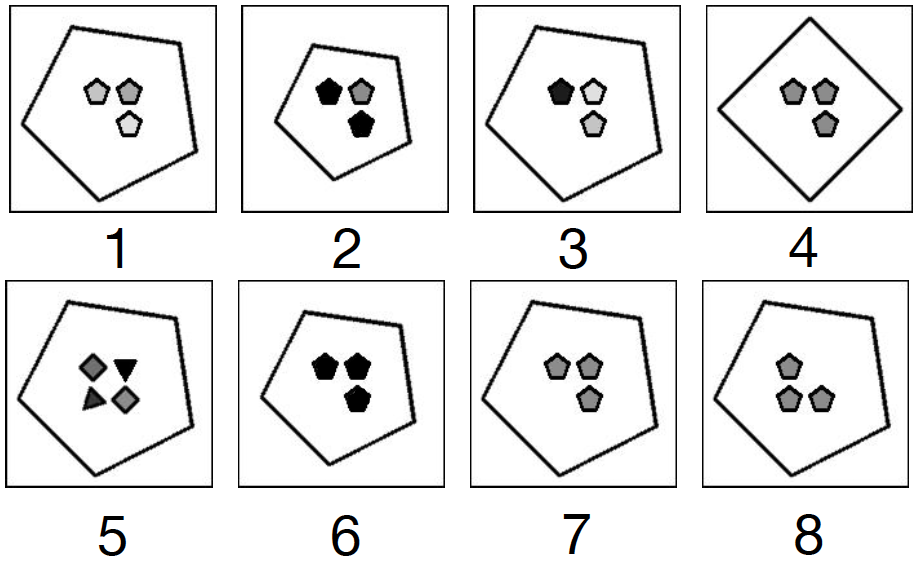
\includegraphics[width=\textwidth]{raven2.png}
        \caption{候选答案}
    \end{subfigure}
    \caption{RAVEN 数据集}
    \label{fig:raven}
\end{figure}

最近,有学者将溯因推理(Abductive Reasoning)引入到自然语言领域,构建了一个新的推理任务:溯因自然语言推理\cite{bhagavatula2019abductive}(Abductive Natural Language Inference, $\alpha$NLI)。图~\ref{fig:aNLI}~是$\alpha$NLI任务的一个示意图。在这个任务中,模型首先可以看到两个观测$O_1$和$O_2$,这两个观测分别表示起始状态和结束状态。
\begin{figure}[!h]
    \centering
    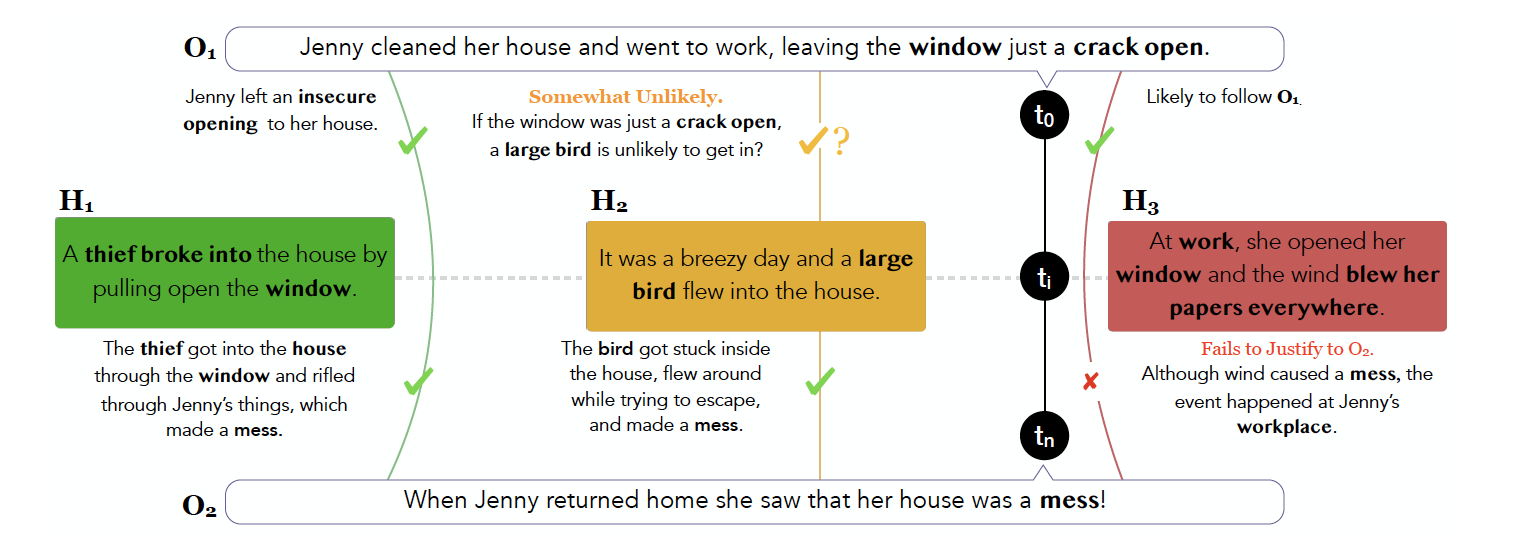
\includegraphics[width=\textwidth]{abductive.png}
    \caption{$\alpha$NLI 任务示意图}
    \label{fig:aNLI}
\end{figure}
例如在图~\ref{fig:aNLI}~中,开始状态为“Jenny 打扫房间后去工作,窗户开了个缝”,结束状态为“Jenny回家时看到房间里一团糟”。模型需要从多个可能的假设$\{H_i\}$中选出最有可能的一个,例如这个例子中展示了三个可能的假设,其中最有可能的假设是“一个小偷从窗户闯入了房子”,而另外两个假设存在明显的逻辑错误。综上可知,在溯因推理任务中,模型需要能够判断出是哪些因素导致了从初始状态到结束状态的变化。

本文提出的视频溯因常识推理就是基于溯因推理的框架而构建的,不同的是在本文提出的任务中,所有的观测和假设都是视觉信息(图片或视频)。这些图片或视频都来自于真实世界,而不是人工合成的,所以需要模型能够具备一定的理解常识的能力。
\section{教程类视频}
教程类视频是在互联网上广泛存在的一类视频,用于指导人们完成生活中的一些简单的任务。教程类视频中往往具有很明确的步骤划分,从而使其具有比普通视频更广泛的应用,例如步骤定位,动作分割、过程规划等等。通过利用视频中的解说信息,还可以实现视频表示的弱监督学习\cite{miech2019end}。一些教程类视频的数据集包括YouCook2\cite{zhou2018towards}、CrossTask\cite{zhukov2019cross}等等。最近,Tang~\etal\cite{tang2019coin}提出了一个新的教程类数据集COIN。该数据集中具有11,827个视频,总时长超过476h。图~\ref{fig:coin}~展示了COIN数据集中样例的标注形式。COIN的标注一共分为三个等级:域(Domain)、任务(Task)、步骤(Step)。其中域表示视频的广义上的分类,例如家务、车辆等等;任务表示视频具体的内容,例如换门把手、换轮胎等等;而步骤则表示了每个动作的名称,例如在换轮胎的任务中,步骤包括“拧下螺丝”、“抬起车子”、“取下轮胎”、“换上轮胎”、“拧紧螺丝”。

由于COIN数据集具有较多的视频和明确的步骤标注,非常适合应用在视频溯因常识推理的任务上。本文以COIN数据集为基础,并对其进行二次标注,构建了视频溯因常识推理的数据集VideoABC。

\begin{figure}[!h]
    \centering
    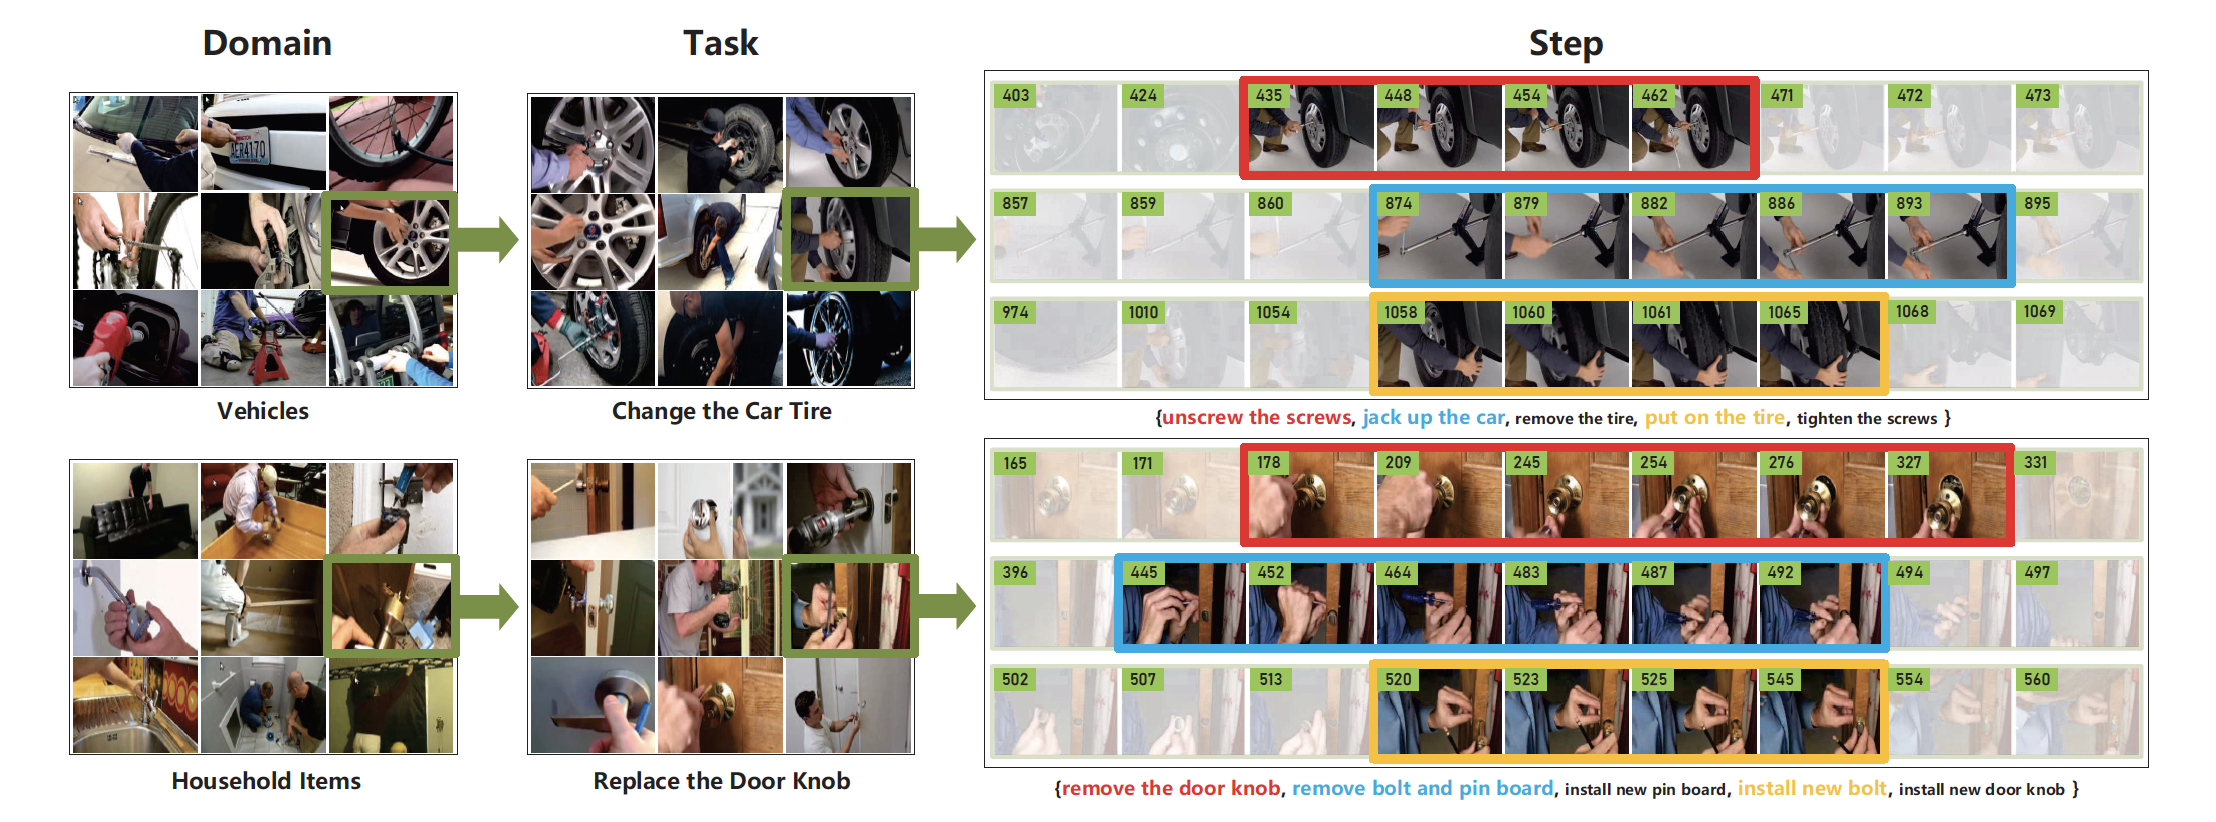
\includegraphics[width=\textwidth]{coin.png}
    \caption{COIN数据集}
    \label{fig:coin}
\end{figure}
\section{视频理解}
从 AlexNet\cite{krizhevsky2012imagenet}开始,卷积神经网络(CNN)就广泛地应用在各种计算机视觉任务中。Karpathy~\etal\cite{karpathy2014large} 提出了利用CNN来提取特征,并在不同的分辨率将特征逐步将融合。为了更好地利用时序信息,Donahue~\etal\cite{donahue2015long} 提出使用LSTM来实现对不同帧特征的融合。另一种应用时序信息的方法是将光流信息作为输入。Simonyan 与 Zisserman\cite{simonyan2014two}提出了一个两分支网络,其中一个分支使用单帧图片作为输入,而另一个分支使用多个光流作为输入,最后将两个分支的预测结果结合。Tran~\etal\cite{tran2015learning}提出使用3D卷积(C3D)来学习时间和空间的特征。为了更好地利用在Imagenet\cite{deng2009imagenet}上预训练的模型,Carreira 与 Zisserman\cite{carreira2017quo}提出通过在时间维度上重复参数将2D卷积直接扩展为3D卷积,并设计了一种新的网络结构I3D(Inflated 3D ConvNet),从而可以在利用时序信息的同时降低训练的难度。Tran~\etal\cite{tran2018closer} 探索了不同类型卷积的组合模式,通过改变将2D和3D卷积的构成,得到了R2D(2D 残差网络)、R3D(3D 残差网络)、MC$x$(混合卷积的残差网络)等结构;通过将
并通过将卷积在时间和空间维度上分解得到了R(2+1)D网络。另一类方法是利用2D卷积网络在等间隔抽帧的视频里提取特征,再通过池化的方式融合特征,即TSN\cite{wang2016temporal}(Temporal Segment Network)。为了更好地挖掘时序关系,Zhou~\etal 在此基础上提出了使用关系网络来对特征进行融合,并使用多级的结构增强鲁棒性。

